\documentclass[conference]{IEEEtran}
\usepackage[UTF8]{ctex}
\usepackage{graphicx}
\usepackage{setspace}
\usepackage{times}
\usepackage{epsfig}
\usepackage{graphicx}
\usepackage{amsmath}
\usepackage{amssymb}
\usepackage{subfigure}
\usepackage{overpic}
\usepackage{stfloats}
\usepackage{array}
\setmainfont{TeX Gyre Termes}

%定义引用
\newcommand{\figref}[1]{图\ref{#1}}
\newcommand{\tabref}[1]{表\ref{#1}}
\newcommand{\equref}[1]{式\ref{#1}}
\newcommand{\secref}[1]{第\ref{#1}节}


%题目信息
\title{无人机集群路径规划}
\author{71121139 孔晔
    09021232 薛沛林
    09021230 孙彦林
    71121140 杨政贤}
\date{\today}



\begin{document}%文章开始


\maketitle%题目



\begin{abstract}%摘要

    近年来,智能无人系统发展迅猛,出现了无人机等一系列新产品,并由此促进了智能无人集群系统的发展。智能无人集群系统将大大提高个体行为的智能化程度,更好地完成单个个体无法完成的工作。对于以灵活机动为特点的无人飞行器(UAV)集群而言,立体空间中的路径规划无疑是重中之重。本小组依托该领域综述性论文,拓展研究了多种路径规划算法,并对无人机集群路径规划研究的意义与未来方向进行讨论。

\end{abstract}




\begin{IEEEkeywords}%关键词

    无人机三维路径规划,
    基于抽样的基本算法,
    基于节点的基本算法,
    基于生物启发的优化算法,
    集群路径规划

\end{IEEEkeywords}


\section{引言}%Section 1 引言

近年来,智能无人系统发展迅猛,出现了无人机、无人车、无人船、无人潜航器、机器人等一系列新产品。智能无人集群系统指若干无人系统根据任务分工,在一定时间、空间内协同完成复杂任务的整体系统。智能无人集群系统具有单个无人系统不可比拟的优势,在农业、制造业、交通、教育、医疗、军事、金融等多个领域具有广阔的应用前景。我们小组这次研究的是智能无人集群系统中应用最为广泛的无人机集群。

集群的研究起始于1959年法国生物学家Pierre Paul Grasse,研究发现昆虫之间存在高度结构化组织,能够群体协同完成远远超出个体能力的复杂任务,这种行为称为群集行为。群集指能够与其他个体以及周围环境交互作用的若干个体集合,如蚁群、鱼群、蜂群等等,它们的简单或微观行为的结合会导致更为复杂和宏观的行为,从而使整个群集行为整体上取得显著效果。

集群并不是对多个个体进行简单的连接和组合,而是使众多个体高效协作、紧密耦合,构成自组织、高稳定的分布式系统,激发个体智慧﹐汇聚群体智能。集群技术将大大提高个体行为的智能化程度,更好地完成单个个体无法完成的工作,通过群体信息共享,扩大对环境态势的感知,实现协同任务分配与协调,能够有效提高群体完成复杂任务的能力,并具有高效率、高容错性和内在的并行性等优点。

无人系统指平台上无需人工操作的物理信息系统,作用于物理世界来完成目标任务。无人系统是由机械、控制、计算机、通信、材料以及人工智能等多种技术融合而成的复杂系统,无人化和智能化是无人系统最显著的两个特征。无人系统的智能化是指在特定任务和环境下,无人系统“感知、认知、分析、沟通、计划、决策和执行”的“自主能力”。无人系统可在时间域和空间域根据环境、任务变化进行实时调整并做出判断,在无人或人工辅助情况下完成任务。

\begin{figure}[tbp]
    \centering
    \begin{overpic}[width=0.45\textwidth]{fig/无人集群介绍}
    \end{overpic}
    \caption{智能无人集群系统技术体系}\label{fig:技术体系}
 \end{figure}

在实际应用上,单个无人机系统由于自身动力、功能和性能等方面的限制,无法单独完成复杂任务,如军事作战、地震等自然灾害需要多无人机系统协同任务执行。为解决单个无人系统的局限性问题,需以集群方式来解决。由此,智能无人机集群是指由一定数量的无人机、控制系统及人机界面组成,利用信息交互与反馈、激励与响应,实现相互间行为协同,适应动态环境,共同完成特定任务的智能联合系统。智能无人机集群不是无人机间的简单组合,而是通过必要的系统集成使之产生集群协同效应,从而具备执行复杂多变、危险任务的能力。因此,智能无人机集群既能最大限度地发挥无人系统的优势,提高整体的载荷能力和信息感知处理能力,又能避免单无人系统执行任务时被能力所限或任务效率不高的问题。

如\figref{fig:技术体系}所示,智能无人集群系统技术体系包括:系统架构、无人平台、通信组网、智能协同和效能评估等五个方面:

系统架构:指从集群系统中各子系统的组成、关联性、交互模式等方面对系统的整体描述。可从信息交互、功能组件、系统部署、系统的关注者等多视角对智能无人集群系统架构进行描述,如从系统部署方式来看,可分为集中式、分布式和混合式。

无人平台:指遥控操作或者自主运作的无人驾驶平台。关键技术包括系统架构、平台本体、动力驱动、载荷接口、自主控制和自主学习等。

通信组网:实现智能无人集群系统各节点间以及系统与外部控制台间的信息交互,关键技术包括大容量、高可靠、抗干扰的传输技术和高效动态组网技术等。

智能协同:指智能无人集群系统通过共享信息联合完成任务的过程,关键技术包括路径规划、协同感知、导航定位、任务规划、协同控制、跨域协同和人机共融。

效能评估:是在一定条件下智能无人集群系统通过智能协同在规定时间内有效完成相应任务效果的综合评价,主要从智能无人集群的自主协同能力、系统鲁棒性、任务效能等方面进行定性和量化评价。

而我们组研究的重点则是智能协调技术体系下无人机及无人机集群的路径规划。


\section{无人机路径规划}%Section 2 无人机路径规划

路径规划是根据智能无人集群系统的工作环境、地理位置、威胁障碍、储能情况等因素,为每个无人系统执行所分配的任务建立可执行的轨迹安排。

智能无人集群系统路径规划的过程涉及众多因素,问题非常复杂,要考虑到特定的目标或者具体任务。从本质上来讲,智能无人集群系统协同路径规划是典型的多目标优化问题,在满足单系统轨迹可适用性要求的同时也要满足整个智能无人集群系统轨迹的协同性要求。目前智能无人集群路径规划常用的研究方法大致可以分为基于纯数学优化的规划方法、基于启发信息的人工智能优化算法和基于生物种群进化的群智能算法。

基于\cite{路径规划数学定义1,路径规划数学定义2,路径规划数学定义3,路径规划数学定义4}的工作,我们可以从数学角度分析无人机路径规划问题。假设无人驾驶飞行器在一个具有障碍物的三维空间$R^3$内飞行。整个空间可记作工作空间$w$。令$wo_i$表示第$i$个障碍物,则无人机可以移动的空间可记为:
\begin{equation}
    w_{free}=w \setminus \cup_i wo_i
\end{equation}

出发点$x_{init}$和目标点$x_{goal}$均是$w_{free}$中的元素,由此我们可以利用$x_{init},x_{goal},w_{free}$定义路径规划问题函数为:
\begin{equation}
    \delta:[0,T]\rightarrow R^3
\end{equation}
其中,$\delta (0)=x_{init}$,$\delta (T)=w_{goal}$,对任意的$\tau \in [0,T]$都有$\delta(\tau) \in w_{free}$。

同时,当我们给定成本函数$c: \sum \rightarrow R \geq0$  $( \sum \mbox{表示所有路径的集合})$后,我们可以定义最优路径$\delta'$使得:
\begin{equation}
    c(\delta')= \min (c(\delta),\delta \mbox{是所有可行路径的集合})
\end{equation}

由此我们得到了无人机路径规划的数学定义。


\subsection{路径规划与轨迹规划的区别与流行算法的介绍}%Subsection 1 路径规划与轨迹规划的区别与流行算法的介绍

从无人机集群的路径规划出发,我们小组找到了一篇该领域的综述性论文A literature review of UAV 3D path planning\cite{无人机路径规划综述}。

轨迹规划是指找到一条平滑连续的轨迹可以绕过障碍物移动。路径规划是时间、空间、能耗等综合下的最优路径。三维空间中的路径规划较二维空间而言需多考虑一个维度,因此其中存在相当多的结构约束和不确定性,特别是在如\figref{fig:三维问题} 所示的森林、洞穴、城市等复杂环境下。简单的二维路径规划算法无法处理复杂的三维环境,无人机导航的三维路径规划算法成为时下之需。

\begin{figure}[htbp]
    \centering
    \begin{overpic}[width=0.45\textwidth]{fig/三维问题}
    \end{overpic}
    \caption{三维空间中的复杂环境}\label{fig:三维问题}
 \end{figure}

 三维环境下的路径规划具有巨大的潜力。但是,与二维规划不同的是,三维环境下的路径规划难度随着动态约束和运动学约束的复杂化呈指数增长。为了在杂乱的环境中规划出一条无碰撞的路径,我们需要运用一些数学方法储存这些数据,并对数据进行建模与约束。因此,从最优化理论的角度来看,寻找一个3D完整路径是一个不存在共同的解决方案的非确定性多项式问题(NP-hard problem)。

 Yang\cite{无人机路径规划综述}将当下流行的算法分为基于抽样的算法、基于节点的算法、基于数学模型的算法基于生物启发的算法四类,并且提出了“基于多重融合算法”这一概念,如\figref{fig:单机规划}所示。

 \begin{figure}[hb]
    \centering
    \begin{overpic}[width=0.45\textwidth]{fig/单机规划}
    \end{overpic}
    \caption{当下流行的算法分类}\label{fig:单机规划}
 \end{figure}

 基于抽样的算法首先将环境作为一组节点进行抽样,然后通过“逐步逼近”或“深度优先搜索”等等过程将节点连接起来。找出所有可能的路径后开始搜索最优路径。这种方法结构简单且易于实现。因此,此算法适用于任一静态或动态的规划条件。
 
 基于节点的算法抛弃了传统的描绘地图的方法转而只处理节点。这种算法通过处理节点信息的方法,将节点之间的距离转化为计算权值,进而直接搜索全局最优路径。这种方法可以与其他方法相结合以实现方法全局最优,适合在动态环境中规划路径。

 基于数学模型的算法旨在通过一种典型的最优化模型描述整个运动空间。它以数学形式描述了几乎所有的动态和运动学约束,并将这些约束与损失函数紧密地绑定在一起。虽然这种方法的计算量总是很大,但随着计算机技术的进步,当代计算机的性能已经足够胜任计算数学模型,因此此方法的效率也随之提高。这些算法并不能实时计算,因此只适合离线工作。

 生物启发算法是一种启发式算法。它能够很好地处理复杂的非结构约束和其他NP问题。这种算法通过突变来优化路径,但突变过程需要较长的迭代时间。因此,这种算法只能离线工作。

 基于多融合的算法将多种算法的优点融合在一起,以实现全局最优和代价最小。此算法通常同时考虑节约时间和信息,有时把几种相对简单的方法结合起来形成一个相对更好的执行方法,因此适合在线实现。
 
\tabref{tab:算法特点}直观展示了这些算法的特点。

\begin{table*}[htbp]
    \centering
    \caption{时下流行算法的特点} \label{tab:算法特点}
    \renewcommand\arraystretch{1.8}
    \resizebox{\textwidth}{!}{
    \begin{tabular}{ l | p{8cm} c c c}
        算法类别&对应算法&时间复杂度&环境&是否实时\\
        \hline
        基于抽样的算法&Voronoi , RRT , PRM, K-PRM , S-PRM , Visibility Graphs , Corridor Map, DDRRT , RRT*&$O(n \log n) \leq T \leq O(n^{2} )$&静态和动态&是\\
        基于节点的算法&Dijkstra’s Algorithms , A* , D*, LPA , Theta* , Lazy Theta* , D*-Lite , Harmony Search&$O(m \log n) \leq T\leq O(n^2)$&静态和动态&是\\
        基于数学模型的算法&Optimal Control , Mixed- Integer Linear Programming , Binary Linear Programming, Non-linear Programming&取决于多项式方程&静态和动态&否\\
        基于生物启发的算法&NN , genetic algorithm , memetic algorithm, particle swarm optimization , ant colony optimization, shuffled frog leaping algorithm&$T \geq O(n^2)$&静态&否\\
        基于多重融合的算法&VVP, PRM Node based, optimal algorithms ,GIS-MCDA algorithms ,visibility graph Node based optimal algorithms , visibility graph ,Geodesics algorithm&$O(n \log n) \leq T$&取决于算法&是
    \end{tabular}
    }
\end{table*}

下面将着重讲解其中的几种代表性算法。

\subsection{基于抽样的基本算法与基于节点的基本算法}%Subsection 2 基于抽样的基本算法与基于节点的基本算法
\subsubsection{Dijkstra算法}%Subsubsection 1  Dijkstra算法

Dijstra是从一个顶点到其余各顶点的最短路径算法,解决的是有权图中最短路径问题。迪杰斯特拉算法主要特点是从起始点开始,采用贪心算法的策略,每次遍历到始点距离最近且未访问过的顶点的邻接节点,直到扩展到终点为止。

查阅资料后,我们举出一下例子以便于理解:

将该算法简单理解为:每次从“未求出最短路径的点”中取出距离距离起点最小路径的点,以这个点为桥梁刷新“未求出最短路径的点的距离”。以$A$点为顶点,求到其他点的最短路径。

$result$:已求出最小路径的顶点

$notFound$:未求出最小路径的顶点,里面的值是到起点的距离

初始如\figref{fig:Dijkstra算法1}所示,$result={A(0)}$中只有起点A,$notFound={B(2),C(\infty),D(6)}$ 中是除了$A$点的其他点,里面的值是到起点的距离(例如$B(2)$代表$B$点到起点的距离为2)

\begin{figure}[htbp]
    \centering
    \begin{overpic}[width=0.45\textwidth]{fig/Dijkstra算法1}
    \end{overpic}
    \caption{Dijkstra算法举例1}\label{fig:Dijkstra算法1}
 \end{figure}

 从“未求出最短路径的点”$notFound$中取出最短路径的点$B(2)$,放入结果$result$中,结果如下:

 “未求出最短路径点”$notFound={C(\infty),D(6)}$

 “已求出最短路径的点”$result={A(0),B(2)}$

 通过$B(2)$为桥梁,刷新距离。

 例如$AD = 6 < AB + BD = 4$以$B(2)$为桥梁的距离更短,就刷新“未求出最短路径点”$D(6)$ 的距离为 $D(4)$,$notFound={C(∞),D(4)}$。

 同理刷新 C(∞) 的距离为 C(5) ,最后结果如下,见\figref{fig:Dijkstra算法2}:

 “未求出最短路径点”$notFound={C(5),D(4)}$

 “已求出最短路径的点”$result={A(0),B(2)}$
 
 \begin{figure}[htbp]
    \centering
    \begin{overpic}[width=0.45\textwidth]{fig/Dijkstra算法2}
    \end{overpic}
    \caption{Dijkstra算法举例2}\label{fig:Dijkstra算法2}
 \end{figure}

 然后,从“未求出最短路径的点”$notFound$中取出最短路径的点$D(4)$,然后通过$D(4)$为桥梁刷新“未求出最短路径的点”的距离。
 同理,最后结果如下,见\figref{fig:Dijkstra算法3}:

 “未求出最短路径点”$notFound={C(5)}$

 “已求出最短路径的点”$result={A(0),B(2),D(4)}$
 
 \begin{figure}[htbp]
    \centering
    \begin{overpic}[width=0.45\textwidth]{fig/Dijkstra算法3}
    \end{overpic}
    \caption{Dijkstra算法举例3}\label{fig:Dijkstra算法3}
 \end{figure}

 然后,从“未求出最短路径的点”$notFound$中取出最短路径的点$C(5)$,算法结束。$result={A(0),B(2),D(4),C(5)}$就是最终所求的最短距离。结果如\figref{fig:Dijkstra算法4}。
 
 \begin{figure}[htbp]
    \centering
    \begin{overpic}[width=0.45\textwidth]{fig/Dijkstra算法4}
    \end{overpic}
    \caption{Dijkstra算法举例4}\label{fig:Dijkstra算法4}
 \end{figure}

 而如果想要知道最短路径,只需要在每个点从$notFound$状态变为$result$状态时,即实现最小距离时连接的前一个点。这样只需要从终点向前连接记录的点,便可以找到最短路径。

\subsubsection{PRM算法}%Subsubsection 2  PRM算法

PRM算法即概率路图算法(Probabilistic Road Map),基于随机采样的路径规划算法。这类算法适用于高维度空间,它们以概率完备性(当时间接近无限时一定有解)来代替完备性,从而提高搜索效率。在阅读论文Path planning using lazy PRM\cite{PRM算法}和查阅有关资料后,我们对PRM有了如下的简单理解。

PRM算法首先使用随机采样的方式在环境中建立路径网络图,将连续的空间转换为离散的空间,然后在路径网络图上进行路径规划,解决在高维空间中搜索效率低的问题。算法流程如下,见\figref{fig:PRM算法流程}:

\begin{figure*}[!t]
    \centering
    \subfigure[采样] {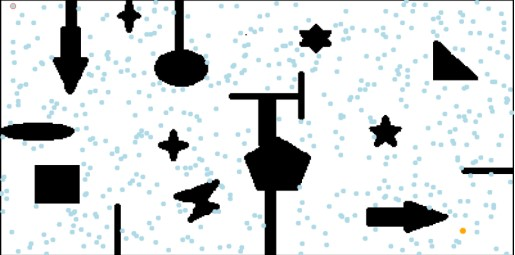
\includegraphics[height=2in,width=2in,angle=-90]{fig/PRM算法1}}
    \subfigure[生成概率路图] {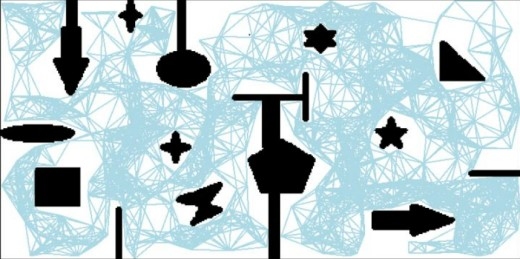
\includegraphics[height=2in,width=2in,angle=-90]{fig/PRM算法2}}
    \subfigure[搜索路径] {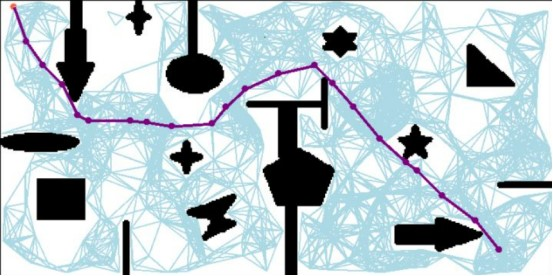
\includegraphics[height=2in,width=2in,angle=-90]{fig/PRM算法3}}
    \caption{ PRM算法流程 }
    \label{fig:PRM算法流程}
\end{figure*}

采样:在地图中随机撒点,剔除落在障碍物上的点。

生成概率路图:根据点与点间的距离和是否存在直线通路将上步中得到的采样点进行连接。

搜索路径:使用图搜索算法(如Dijkstra算法)在上步得到的路图中搜索出一条从起点到终点的最短路径。

其中采样点的数量和采样点间存在通路的最大距离是路径规划成功与否的关键。

采样点太少,可能会导致路径规划失败;

采样点数量增加,搜索到的路径会逐渐接近最短路径,但同时搜索效率会降低。

PRM算法参数少、结构简单,能够提高高维空间搜索效率,也能在生成概率路图时添加机器人的运动学约束,使最终生成的路径符合机器人的运动学模型。同时,随机采样得到的概率路图只需要建立一次就可以一直使用,重用性强。但由于采样过程是完全随机的,得到的节点大多数都偏离最终路径,会增加额外的计算量。

\subsubsection{RRT算法}%Subsubsection 3  RRT算法

RRT即快速随机扩展树算法(Rapidly-exploring Random Tree, RRT)

RRT算法是一种单查询(single-query)算法,目标是尽可能快的找到一条从起点到终点的可行路径。在阅读了论文Rapidly-Exploring Random Trees: A New Tool for Path Planning\cite{RRT算法}和查阅了部分资料后,我们将改算法简单理解为下面几个步骤:

如\figref{fig:RRT算法1},它的搜索过程类似于一棵树不断生长、向四周扩散的过程,它以起点作为根节点构建一棵搜索树$T$。

\begin{figure}[htbp]
    \centering
    \begin{overpic}[width=0.45\textwidth]{fig/RRT算法1}
    \end{overpic}
    \caption{RRT算法图示}\label{fig:RRT算法1}
\end{figure}

用$X_{init}$ 表示起点,$T$表示随机树,在算法开始时,将起点$X_{init}$加入到随机树。接下来使用$SampleFree$函数在自由空间中随机采样,获得一个采样点$X_{rand}$,再使用$Nearest$函数获得随机树中距离$X_{rand}$最近的一个节点$X_{near}$;使用$Steer$函数在$X_{near}$和$X_{rand}$的连线上距离$X_{near}$步长$u$的位置生成一个节点$X_{new}$,使用$ObtacleFree$函数判断$X_{near}$和$X_{new}$间是否存在直线通路,若存在则将$X_{new}$加入到随机树$T$的节点集合中,同时将$X_{near}$作为$X_{new}$的父节点,将边$ (X_{near},X_{new})$加入到随机树$T$的边集中。

\begin{figure}[htbp]
    \centering
    \begin{overpic}[width=0.45\textwidth]{fig/RRT算法2}
    \end{overpic}
    \caption{RRT算法原理}\label{fig:RRT算法2}
\end{figure}

在自由空间中随机采样得到采样点$X_{rand}$,从搜索树$T$中找出距离采样点$X_{rand}$最近的节点$X_{near}$计算$X_{near}$和$X_{rand}$之间的距离。如果距离大于步长$u$,则从$X_{near}$向$X_{rand}$移动步长$u$后得到新节点$X_{new}$;否则在$X_{rand}$位置生成新节点$X_{new}$. 如果$X_{new}$和$X_{near}$间存在直线通路,则将$X_{new}$加入搜索树$T$,它的父节点为$X_{near}$;否则进入下一轮循环。

上述是基础的RRT算法流程,\figref{fig:RRT算法2}给出了算法的图片解释。该算法的采样过程是完全随机的,还可以在采样时以一定的概率直接采样终点作为$X_{rand}$,加快搜索速度。

RRT作为一种随机采样的规划算法,它的复杂度也不受地图的离散程度影响,在高维空间中仍具有很高的搜索效率。但是前面提到RRT是一种单查询算法,只管尽快地找到可行路径,所以最终路径并不是最优的,甚至会非常“绕”。

此外,还有一些基于RRT的优化算法,例如RRT-connect、RRT*等,可以参考这些论文RRT-connect: An efficient approach to single-query path planning\cite{基于RRT的优化算法1}、Sampling-based Algorithms for Optimal Motion Planning\cite{基于RRT的优化算法2}。

\subsection{基于生物启发的优化算法}%Subsection 3 基于生物启发的优化算法

生物优化算法起源于模仿生物行为来对路径进行规划,该路径规划的方法省略了构建复杂环境模型的过程,是一种稳定的收敛到目标的强搜索方法。在生物启发的优化算法中,存在多种不同的道路,例如:遗传算法\cite{生物启发4}、模因算法\cite{生物启发5}、蚁群算法\cite{生物启发1,生物启发2}、蛙跳算法\cite{生物启发6}等等。求解路径规划可分为精确算法和人工智能算法,精确算法基于严格的数学手段,在可求解的情况下解的质量较好,但算法严格,运算量大,在大规模的问题上几乎无法求解,而人工智能算法基本在可接受的时间里找到可接受的满意解,此情况中基于生物启发的优化算法就属于人工智能算法。在此小节之中,我将会简单讲解生物启发算法蚁群算法以及优化后的精英蚁群算法。

\figref{fig:基于生物启发的优化算法}展示了蚁群算法的基本原理:
\begin{enumerate}
    \item 蚂蚁在路径上释放信息素
    \item 碰到还没走过的路口,随机挑选一条路走。同时释放与路径长度相关的信息素,信息素浓度与路径长度成反比
    \item 后来的蚂蚁碰到路口时选择信息素浓度较高的路径
    \item 最优路径上的信息素浓度越来越大
    \item 最终找到最优寻食路径
\end{enumerate}

\begin{figure}[htbp]
    \centering
    \begin{overpic}[width=0.45\textwidth]{fig/基于生物启发的优化算法}
    \end{overpic}
    \caption{蚁群算法的基本原理}\label{fig:基于生物启发的优化算法}
 \end{figure}

 在无人机路径规划中使用蚁群算法则需先获取环境情况,将其进行一个简单建模,确定起点与终点,开始进行蚁群算法的迭代,经过多次迭代后所获得的信息素浓度最高的那一条路径即为最优路径。

 然而我们通过蚁群算法的规则可以知道,当问题的规模很大的时候,蚁群算法的性能会急速下降,并且解的总质量提高了,但是解元素之间的差异减少了,导致选择概率的差异随之减小,搜索过程会集中在目前最优解附近,而不一定是全局的最优解。对此提出了一些优化算法。

 一种是精英蚁群算法,通过给本次迭代最优解赋予额外信息素的方式,可以加快算法的收敛,本次迭代中寻找到最优解的即为精英蚂蚁。

 另一种是基于优化排序的蚂蚁系统,在普通的蚂蚁系统上给信息素的释放加上了一个权值,只有生成了至今最优路径的蚂蚁和路径长度排名靠前的蚂蚁才被允许释放信息素,且排名越靠前的蚂蚁可以释放的信息素越多,这样就有效避免蚂蚁集中于当前最优线路导致其他对全局最优线路搜寻的忽视。

 整个生物优化的启发算法类似于机器学习人工智能中的算法,我对此的了解并不是很深也不一定正确,这方面算法相关内容也非常欢迎人智的同学来进行一些补充。传统的遗传进化方法可能已经达到了瓶颈阶段。相比之下,随着深度学习技术的发展,越来越多的研究人员开始将机器学习和深度学习技术应用于无人机路径规划。\cite{生物启发3}
 
\subsection{集群路径规划}%Subsection 4 集群路径规划




\section{总结}%Section 3 总结



\subsection{文章结构及论文关系}%Subsection 1 文章结构及论文关系



\subsection{工作意义}%Subsection 2 工作意义



\subsection{未来研究方向}%Subsection 3 未来研究方向[1]



\subsection{欠缺之处}%Subsection 4 欠缺之处


%参考文献
\bibliographystyle{IEEEtran}
\bibliography{ref.bib}

\end{document}
